\documentclass[journal,12pt,twocolumn]{IEEEtran}

\usepackage{setspace}
\usepackage{gensymb}

\singlespacing


\usepackage[cmex10]{amsmath}

\usepackage{amsthm}

\usepackage{mathrsfs}
\usepackage{txfonts}
\usepackage{stfloats}
\usepackage{bm}
\usepackage{cite}
\usepackage{cases}
\usepackage{subfig}

\usepackage{longtable}
\usepackage{multirow}

\usepackage{enumitem}
\usepackage{mathtools}
\usepackage{steinmetz}
\usepackage{tikz}
\usepackage{circuitikz}
\usepackage{verbatim}
\usepackage{tfrupee}
\usepackage[breaklinks=true]{hyperref}
\usepackage{graphicx}
\usepackage{tkz-euclide}

\usetikzlibrary{calc,math}
\usepackage{listings}
    \usepackage{color}                                            %%
    \usepackage{array}                                            %%
    \usepackage{longtable}                                        %%
    \usepackage{calc}                                             %%
    \usepackage{multirow}                                         %%
    \usepackage{hhline}                                           %%
    \usepackage{ifthen}                                           %%
    \usepackage{lscape}     
\usepackage{multicol}
\usepackage{chngcntr}

\DeclareMathOperator*{\Res}{Res}

\renewcommand\thesection{\arabic{section}}
\renewcommand\thesubsection{\thesection.\arabic{subsection}}
\renewcommand\thesubsubsection{\thesubsection.\arabic{subsubsection}}

\renewcommand\thesectiondis{\arabic{section}}
\renewcommand\thesubsectiondis{\thesectiondis.\arabic{subsection}}
\renewcommand\thesubsubsectiondis{\thesubsectiondis.\arabic{subsubsection}}


\hyphenation{op-tical net-works semi-conduc-tor}
\def\inputGnumericTable{}                                 %%

\lstset{
%language=C,
frame=single, 
breaklines=true,
columns=fullflexible
}
\begin{document}


\newtheorem{theorem}{Theorem}[section]
\newtheorem{problem}{Problem}
\newtheorem{proposition}{Proposition}[section]
\newtheorem{lemma}{Lemma}[section]
\newtheorem{corollary}[theorem]{Corollary}
\newtheorem{example}{Example}[section]
\newtheorem{definition}[problem]{Definition}

\newcommand{\BEQA}{\begin{eqnarray}}
\newcommand{\EEQA}{\end{eqnarray}}
\newcommand{\define}{\stackrel{\triangle}{=}}
\bibliographystyle{IEEEtran}
\providecommand{\mbf}{\mathbf}
\providecommand{\pr}[1]{\ensuremath{\Pr\left(#1\right)}}
\providecommand{\qfunc}[1]{\ensuremath{Q\left(#1\right)}}
\providecommand{\sbrak}[1]{\ensuremath{{}\left[#1\right]}}
\providecommand{\lsbrak}[1]{\ensuremath{{}\left[#1\right.}}
\providecommand{\rsbrak}[1]{\ensuremath{{}\left.#1\right]}}
\providecommand{\brak}[1]{\ensuremath{\left(#1\right)}}
\providecommand{\lbrak}[1]{\ensuremath{\left(#1\right.}}
\providecommand{\rbrak}[1]{\ensuremath{\left.#1\right)}}
\providecommand{\cbrak}[1]{\ensuremath{\left\{#1\right\}}}
\providecommand{\lcbrak}[1]{\ensuremath{\left\{#1\right.}}
\providecommand{\rcbrak}[1]{\ensuremath{\left.#1\right\}}}
\theoremstyle{remark}
\newtheorem{rem}{Remark}
\newcommand{\sgn}{\mathop{\mathrm{sgn}}}
\providecommand{\abs}[1]{\left\vert#1\right\vert}
\providecommand{\res}[1]{\Res\displaylimits_{#1}} 
\providecommand{\norm}[1]{\left\lVert#1\right\rVert}
%\providecommand{\norm}[1]{\lVert#1\rVert}
\providecommand{\mtx}[1]{\mathbf{#1}}
\providecommand{\mean}[1]{E\left[ #1 \right]}
\providecommand{\fourier}{\overset{\mathcal{F}}{ \rightleftharpoons}}
%\providecommand{\hilbert}{\overset{\mathcal{H}}{ \rightleftharpoons}}
\providecommand{\system}{\overset{\mathcal{H}}{ \longleftrightarrow}}
	%\newcommand{\solution}[2]{\textbf{Solution:}{#1}}
\newcommand{\solution}{\noindent \textbf{Solution: }}
\newcommand{\cosec}{\,\text{cosec}\,}
\providecommand{\dec}[2]{\ensuremath{\overset{#1}{\underset{#2}{\gtrless}}}}
\newcommand{\myvec}[1]{\ensuremath{\begin{pmatrix}#1\end{pmatrix}}}
\newcommand{\mydet}[1]{\ensuremath{\begin{vmatrix}#1\end{vmatrix}}}
\numberwithin{equation}{subsection}
\makeatletter
\@addtoreset{figure}{problem}
\makeatother
\let\StandardTheFigure\thefigure
\let\vec\mathbf
\renewcommand{\thefigure}{\theproblem}
\def\putbox#1#2#3{\makebox[0in][l]{\makebox[#1][l]{}\raisebox{\baselineskip}[0in][0in]{\raisebox{#2}[0in][0in]{#3}}}}
     \def\rightbox#1{\makebox[0in][r]{#1}}
     \def\centbox#1{\makebox[0in]{#1}}
     \def\topbox#1{\raisebox{-\baselineskip}[0in][0in]{#1}}
     \def\midbox#1{\raisebox{-0.5\baselineskip}[0in][0in]{#1}}
\vspace{3cm}
\title{Assignment 4}
\author{Pulkit Saxena}
\maketitle
\newpage
\bigskip
\renewcommand{\thefigure}{\theenumi}
\renewcommand{\thetable}{\theenumi}
\section{Problem(loney pg 98 Q7)}
Find the value of k so that following equation may represent pairs of straight lines,
\begin{align}
12x^2-10xy+2y^2+11x-5y+k=0
\label{1}
\end{align}
\section{Solution}
The general equation of second degree is given by,
\begin{align}
ax^2 + 2bxy + cy^2 + 2dx +2ey +f = 0
\label{2}
\end{align}
In vector from the equation \eqref{2} can be expressed as,
\begin{align}
\vec{x}^T\vec{V}\vec{x} + 2\vec{u}^T\vec{x} + f = 0 
\label{line_vec}
\end{align}
where,
\begin{align}
\vec{V} = \vec{V}^T = \myvec{a&b\\b&c}
\label{3}
\end{align}
\begin{align}
\vec{u} = \myvec{d\\e}
\label{4}
\end{align}
Now, comparing \eqref{2} to \eqref{1} we get, a =12, b=-5, c = 2, d = $\frac{11}{2}$,e = -$\frac{5}{2}$, f = k.  
Hence, substituting these values in \eqref{3} and \eqref{4} we get,
\begin{align}
\vec{V} = \myvec{12 & -5 \\ -5 & 2}
\end{align}
\begin{align}
\vec{u} = \myvec{\frac{11}{2} \\ -\frac{5}{2}}
\end{align}
\eqref{1} represents pair of straight lines if,
\begin{align}
\mydet{\vec{V}&\vec{u}\\\vec{u}^T&f} = 0
\end{align}
\begin{align}
\mydet{12&-5&\frac{11}{2}\\-5&2&-\frac{5}{2}\\\frac{11}{2}&-\frac{5}{2}&k} = 0
\end{align}
\begin{align}
\implies k =2
\label{5}
\end{align}
Lines Intercept if
\begin{align}
    |\vec{V}|<0\\
    |\vec{V}|=-1<0
\end{align}
Hence Line intercept.\\
Let $(\alpha,\beta)$ be their point of intersection, then
\begin{equation}\label{eq6}
	\myvec{ a & b\\ b & c}\myvec{\alpha \\ \beta} = \myvec{-d \\ -e}
\end{equation}
Substituting in \eqref{eq6}
\begin{align}
	\label{eq11}\myvec{ 12 & -5\\-5 & 2}\myvec{\alpha \\ \beta} = \myvec{-\frac{11}{2} \\ \frac{5}{2}} \\
	\label{eq12}\implies \myvec{\alpha \\ \beta} = \myvec{-\frac{3}{2} \\ -\frac{5}{2}}
\end{align}
Spectral Decomposition  of $\vec{V}$ is given as
\begin{equation}
\vec{V} = \vec{P}\vec{D}\vec{P}^T
\end{equation}
\begin{align}
	\label{eq7}\vec{V} &= \myvec{ 12 & -5\\ -5 & 2}\\
	\label{eq8}\vec{P} &= \myvec{-1-\sqrt{2} & -1 + \sqrt{2}\\ 1 & 1}\\
	\label{eq9}\vec{D} &= \myvec{7 + 5\sqrt{2} & 0\\ 0 & 7 - 5\sqrt{2}}
\end{align}
Using Spectral decomposition concept and substution
\begin{align}
u_1(x-\alpha) + u_2(y-\beta) &= \pm \sqrt{-\frac{\lambda_2}{\lambda_1}}(v_1(x-\alpha) + v_2(y-\beta))\label{eq10}
\end{align}
Substituting \eqref{eq12}, \eqref{eq8} and \eqref{eq9} in \eqref{eq10}
\begin{multline}\label{eq13}
	\brak{-1-\sqrt{2}}\brak{x- \frac{-3}{2}} + \brak{y-\frac{-5}{2}} \\= \pm \sqrt{-\frac{7 +5\sqrt{2}} {7-5\sqrt{2}}}\brak{\brak{-1+\sqrt{2}}\brak{x- \frac{-3}{2}} + \brak{y-\frac{-5}{2}}}
\end{multline}
Simplifying \eqref{eq13},
\begin{align}
	\label{eq22}-6x + 2y - 4 = 0 \text{ and } -2x + y -\frac{1}{2} = 0\\
	\implies \brak{-6x + 2y - 4}\brak{-2x + y -\frac{1}{2}} = 0
\end{align}
Thus the equation of lines are
\begin{align}
\myvec{-6&2}\vec{x} = 4\\ 
\myvec{-2&1}\vec{x} = \frac{1}{2}
\end{align}
Hence, Plot is shown below 
\begin{figure}[ht!]
\centering
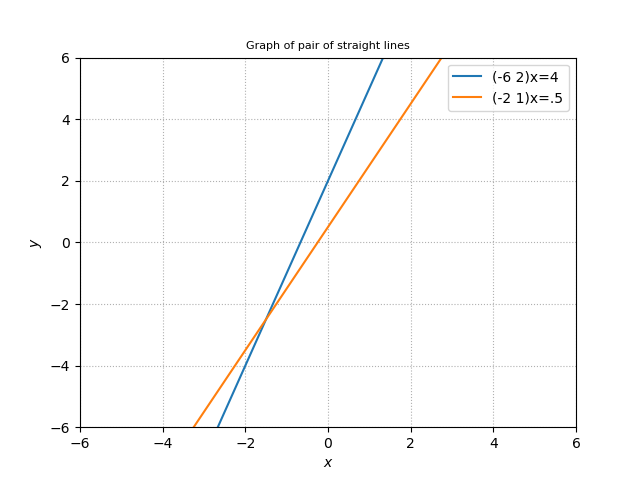
\includegraphics[width=\columnwidth]{Figure.png}
\caption{Pair of lines}
\end{figure}
\begin{comment}
\end{comment}
\end{document}
